% XCircuit output "Voltagedivider.tex" for LaTeX input from Voltagedivider.eps
\def\putbox#1#2#3#4{\makebox[0in][l]{\makebox[#1][l]{}\raisebox{\baselineskip}[0in][0in]{\raisebox{#2}[0in][0in]{\scalebox{#3}{#4}}}}}
\def\rightbox#1{\makebox[0in][r]{#1}}
\def\centbox#1{\makebox[0in]{#1}}
\def\topbox#1{\raisebox{-0.60\baselineskip}[0in][0in]{#1}}
\def\midbox#1{\raisebox{-0.20\baselineskip}[0in][0in]{#1}}
   \scalebox{0.5}{
   \normalsize
   \parbox{2.45312in}{
   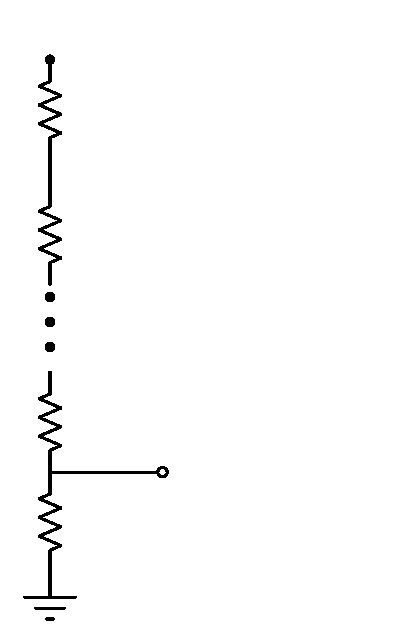
\includegraphics[scale=1]{images/Voltagedivider.eps}\\
   % translate x=208 y=444 scale 0.38
   \putbox{0.31in}{3.87in}{1.20}{$V_{applied}$}%
   \putbox{1.06in}{1.12in}{1.20}{$V_{meaured}$}%
   } % close 'parbox'
   } % close 'scalebox'
   \vspace{-\baselineskip} % this is not necessary, but looks better
